\section{Design entry and the tool bus}
\label{designEntryAndToolBus}

\subsection{Multi-formalism specification}
\label{tool bus}
One of our goals in APEX is to formally verify the safety of the autonomous system's operation in all scenario types.
As we saw in Section \ref{safety}, the imperative to be safe is expressed by different logic properties in the different scenarios types.
For example, in a Crosswalk scenario, one safety-inducing property is ``Pedestrian in crosswalk $\implies$ car is stopped''.
To verify these properties, we must first decide on the appropriate formalism(s) in whic to express them (e.g. LTL, CTL, or MTL?) 
and the corresponding formalism for describing the autonomous system under verification.
Secondly, we must decide on which tool to run to verify the property.
In general, we may expect that different properties, and different levels of abstraction at which they are verified, will require (or be better verified) using different formalisms and tools. 
For example, verifying a property of the continuous-time dynamics may be done using {\staliro}~\cite{AnnapureddyLFS11tacas},
whereas verifying a property of the discrete mission planner may be best done using UPPAAL \cite{BehrmannDLHPYH06qest}.
This motivates the creation of a translator from our detailed HCHA representation of the scenario instance to the different formalisms that are deemed useful. 
For example: timed automata, weighted timed automata, Ordinary Differential Equation (ODEs), impulsive systems,...etc.

\begin{figure}[tb]
	\centering
		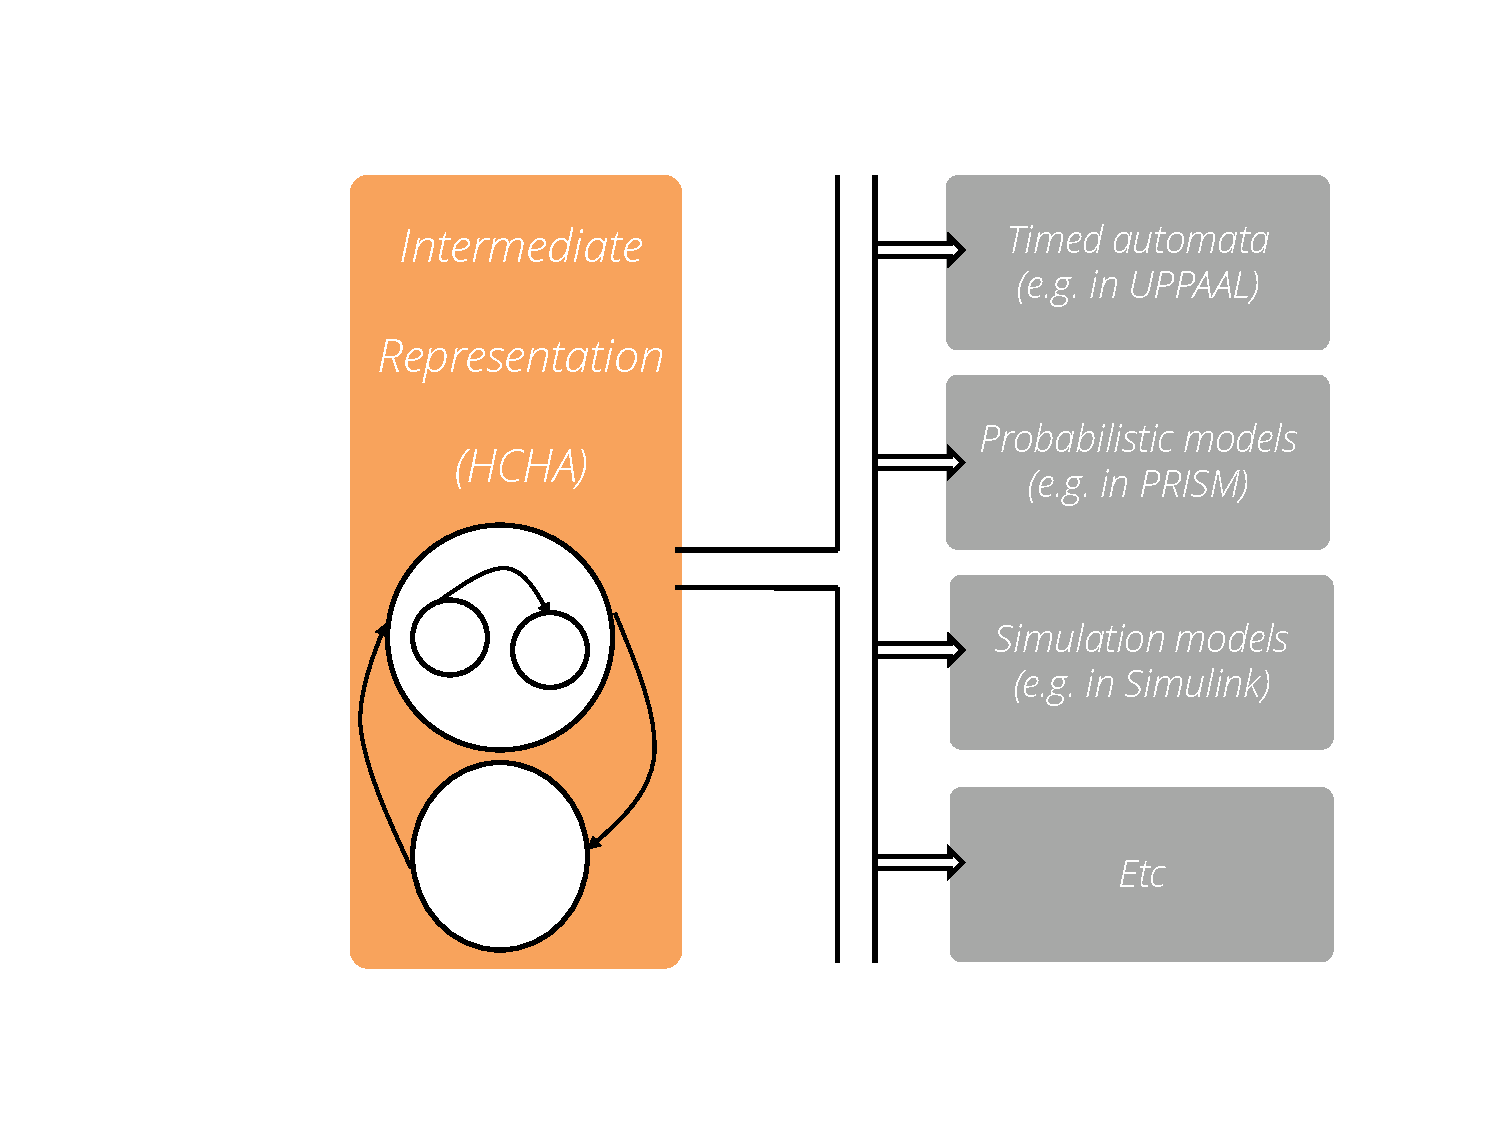
\includegraphics[scale=0.3]{figures/toolbus.pdf}
	\label{fig:toolbus}
	\caption{The APEX tool bus.}
\end{figure}

The representation of a scenario and its agents in some Intermediate Representation (IR) allows the translation into many other formalisms.
The key requirement is that the IR must be at least as detailed as any target formalism.
Formally, we say that a model $\Mc_1$ (in formalism $F_1$, e.g. HCHA) is at least as detailed as model $\Mc_2$ (in formalism $F_2$, e.g. timed automata) if the behavior of $\Mc_2$ contains the behavior of $\Mc_1$: 
\[\behavior_{\Mc_1} \subset \behavior_{\Mc_2}\]
This is the familiar notion of behavior inclusion, and it is one more reason for choosing HCHA as the IR:
the most detailed analysis that can be made on the autonomous system is at the level of the continuous dynamics.
These are captured in the HCHA. 
Other aspects are also captured in the HCHA, as explained in Section \ref{HCHA}.
These details can be abstracted when translating the HCHA to, say, a timed automaton to perform verification using UPPAAL.
On the other hand, had we chosen timed automata as our IR, we would not have been able to recover the true dynamics from the timed automaton's differential inclusions. 
This would preclude us from performing accurate reachability computations for example, or control performance analysis, such as disturbance rejection and stability.

\todo[inline]{a word on jhow to transfer verif results back to HCHA}

To enable push-button formal verification of the safety-inducing properties, APEX includes a \emph{tool bus}; see Fig.~\ref{fig:toolbus}.
Once a combination of tools is decided on for a particular verification task, the IR is translated to the formats of these tools and transmitted to them.

%===============================================================================================================
\subsection{Scenario authoring tool and Domain-Specific Language}
\label{dsl}
\todo[inline]{Matt}
How are the scenarios created? 
Glad you asked: DSL and its formal semantics in terms of HCHA, then scenario authoring tool.
Gesture towards a GUI, possibly in Simulink (APEX-S). 
Emphasize that while nondeterminism of the environment will somehow be expressed in APEX-S, we are NOT simulating with non-determinism. For one thing that's impossible, but just to avoid reviewers scratching their heads over what on Earth we mean.
APEX-S is just an editor. We may leverage it on the tool bus (see previous section), but in and of itself, 'tis an editor.
